\documentclass[aspectratio=169]{beamer}
\setbeamertemplate{navigation symbols}{}
\usepackage{color,amsmath,comment, subfigure}
\usepackage{booktabs}
\usepackage{url}

\def\imagetop#1{\vtop{\null\hbox{#1}}} %http://tex.stackexchange.com/questions/23521/tabular-vertical-alignment-to-top

%%%%%%%%%%%%%%%%%%%%%%%%%%
\title[]{Lecture 23: Who knows what about who?}
\author[]{Matthew J. Salganik}
\institute[]{Sociology 204: Social Networks\\Princeton University}
\date[]{
1/2 Game of contacts and the scale-up method

\vfill

\begin{flushleft}
\vspace{0.6in}
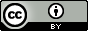
\includegraphics[width=0.1\textwidth]{figures/cc.png}
\end{flushleft}
}

\note{
More compare and contrast of three studies:
- design (interview of alters vs guess what alter will say, game of contacts doesn't ask actual alter info)
- goals (basic vs applied)
}

\begin{document}
%%%%%%%%%%%%%%%%%%%%%%%%%%%
\frame{\titlepage}
%%%%%%%%%%%%%%%%%%%%%%%%%%%
% %%%%%%%%%%%%%%%%%%%%%%%%
\begin{frame}

\begin{center}
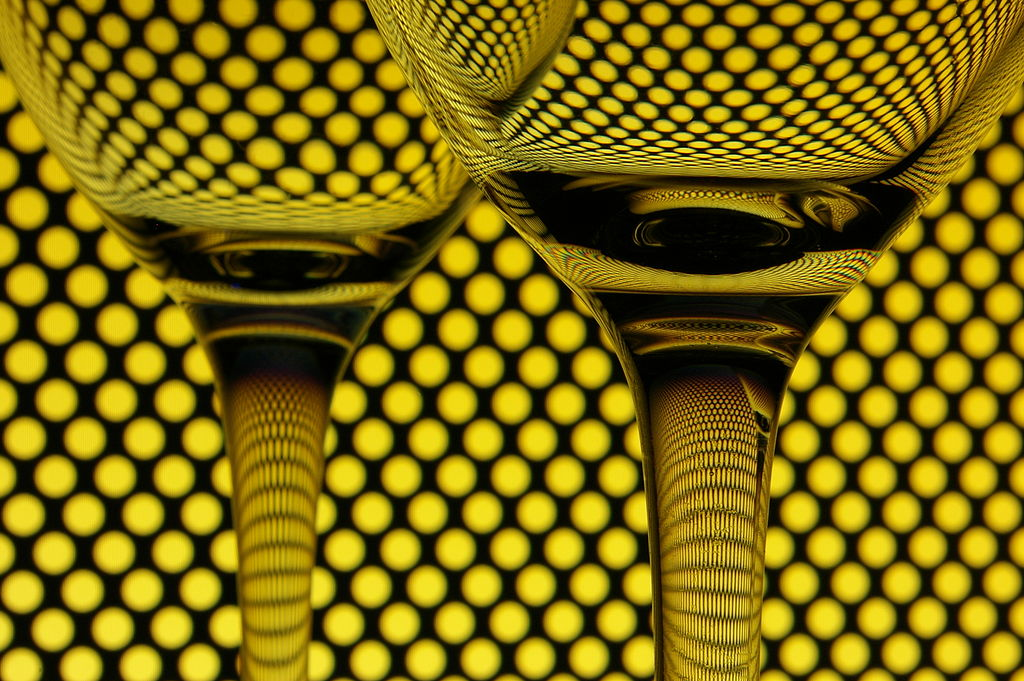
\includegraphics[width=0.8\textwidth]{figures/distortion.jpg}
\end{center}

\vfill
\tiny{\url{https://commons.wikimedia.org/wiki/File:Uniformity.jpg}}

\note{
What you see is distorted
}

\end{frame}
%%%%%%%%%%%%%%%%%%%%%%%%%%%
\begin{frame}

\begin{itemize}
\item your perception of the social world is distorted
\pause
\item your perception of your own social world is distorted
\end{itemize}

\pause 
Why do we care?

\begin{itemize}
\item important for scale-up method
\end{itemize}

\end{frame}
%%%%%%%%%%%%%%%%%%%%%%%
\begin{frame}

\begin{center}
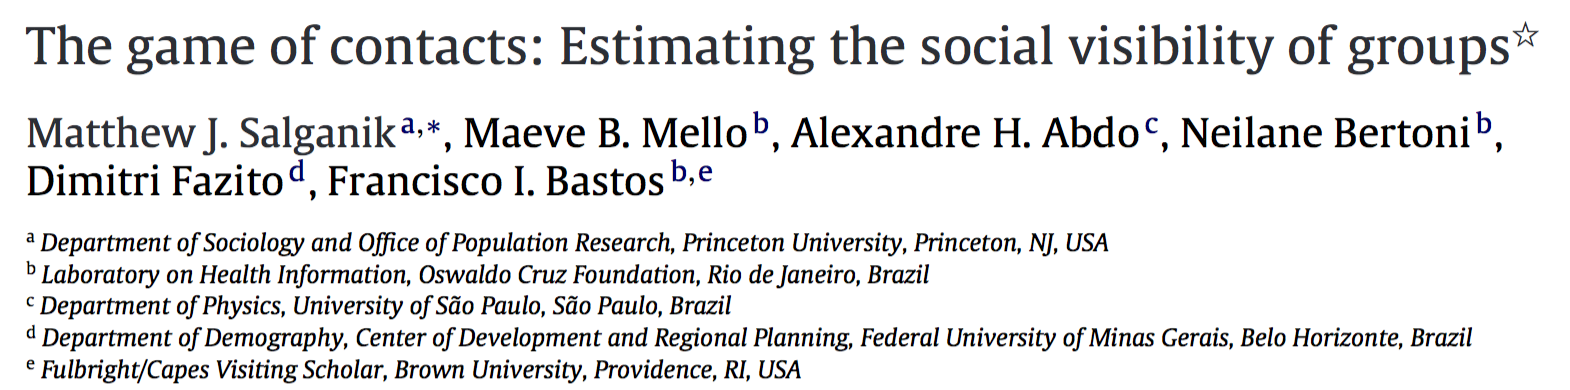
\includegraphics[width=0.9\textwidth]{figures/salganik_game_2011_title.png}
\end{center}

\end{frame}
%%%%%%%%%%%%%%%%%%
\begin{frame}

\begin{itemize}
\item Hidden population: Heavy drug users, people who had used illegal drugs other than marijuana more than 25 times in the past 6 months
\item Location: Curitiba, Brazil (1.8 million people)
\item Funded by UNAIDS and Brazilian Ministry of Health
\end{itemize}

\framebox{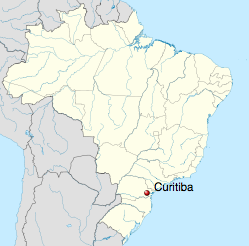
\includegraphics[width=0.3\textwidth]{figures/curitiba_on_map_wikipedia}}\\
\tiny{Map source: Wikipedia}

\end{frame}
%%%%%%%%%%%%
\begin{frame}

We want to learn about:
\begin{itemize}
\item true positive rate (probability that a randomly chosen alter of a randomly chosen ego in the hidden population is aware that ego is in the hidden population) \pause
\end{itemize}

\end{frame}
%%%%%%%%%%%%%
\begin{frame}

Interviewer shuffles a deck of 24 playing cards
\vfill
\begin{center}
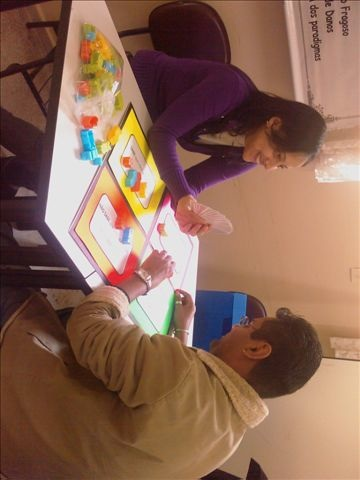
\includegraphics[angle=90, width=0.7\textwidth]{figures/jogo_drawcards}
\end{center}

\end{frame}
%%%%%%%%%%%%%
\begin{frame}

A card is pulled from the deck and the respondent is asked:

\begin{columns}[c]
\column{2in}
\begin{center}
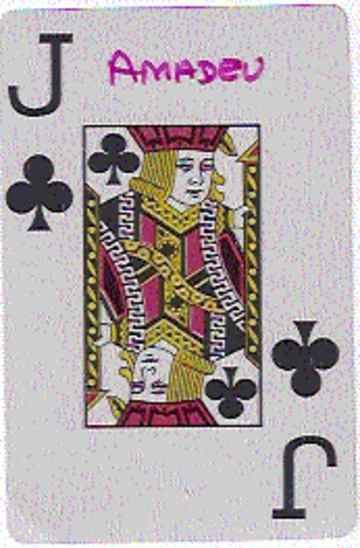
\includegraphics[height=2in]{figures/amadeu_card}
\end{center}

\column{3in}
How many people do you know named [Amadeu]?
\end{columns}

\end{frame}
%%%%%%%%%%%%
\begin{frame}

The respondent will pick up this many blocks and place them:\\
\begin{center}
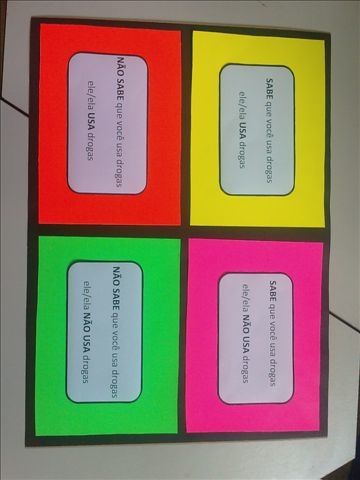
\includegraphics[angle=90, width=0.6\textwidth]{figures/jogo_board}
\end{center}
\vfill
Record answers; clear board; repeated for 24 names. 

\end{frame}
%%%%%%%%%%%%
\begin{frame}

\begin{center}
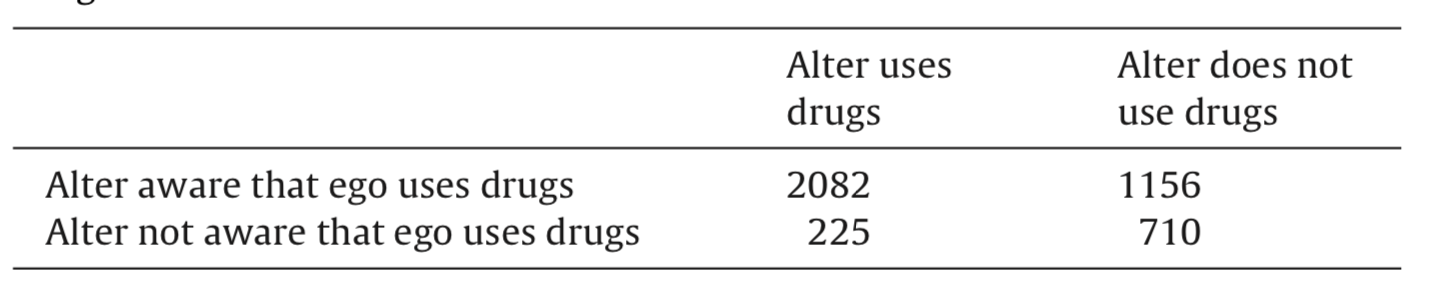
\includegraphics[width=\textwidth]{figures/salganik_game_2011_tab2}
\end{center}

\begin{itemize}
\item Overall
\begin{equation*}
 \hat{\tau} = \frac{ \textrm{total alters aware} }  {\textrm{total alters}} = \frac{3,238}{4,173} = 0.78 
\end{equation*}
\pause
\item Alter uses drugs
\begin{equation*}
 \hat{\tau} = \frac{ \textrm{total alters aware} }  {\textrm{total alters}} = \frac{2,082}{2,307} = 0.90 
\end{equation*}
\pause
\item Alter does not use drugs
\begin{equation*}
 \hat{\tau} = \frac{ \textrm{total alters aware} }  {\textrm{total alters}} = \frac{1,156}{1,866} = 0.62 
\end{equation*}
\end{itemize}

\vfill
{\tiny Estimates slightly different from paper because estimates in paper include sampling weights (which are neglected here for simplicity)}

\end{frame}
%%%%%%%%%%%%%
\begin{frame}

\begin{center}
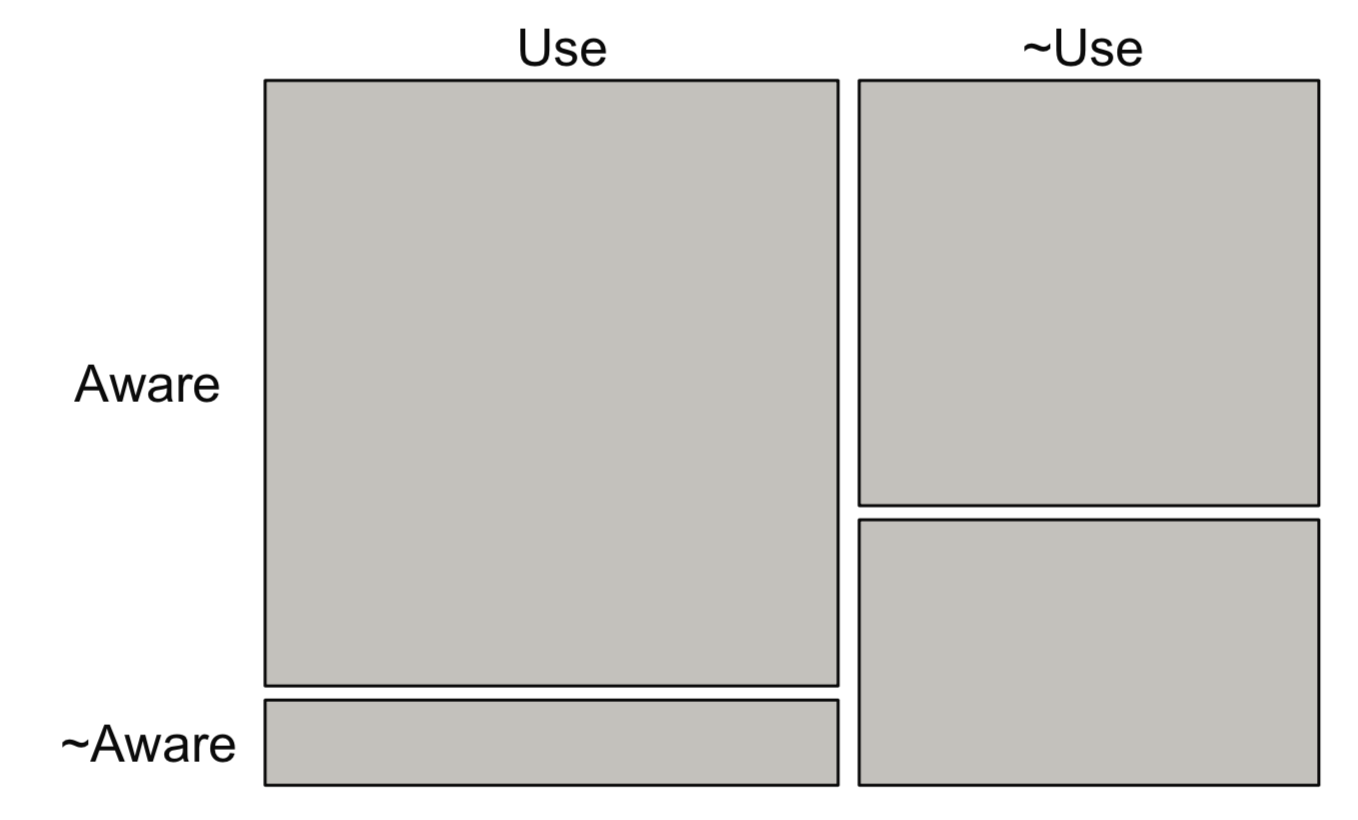
\includegraphics[width=0.5\textwidth]{figures/salganik_game_2011_fig3}
\end{center}

\vfill
Evidence of:
\begin{itemize}
\item selective exposure \pause
\item selective disclosure
\end{itemize}

\end{frame}
%%%%%%%%%%%%%
\begin{frame}

\begin{center}	
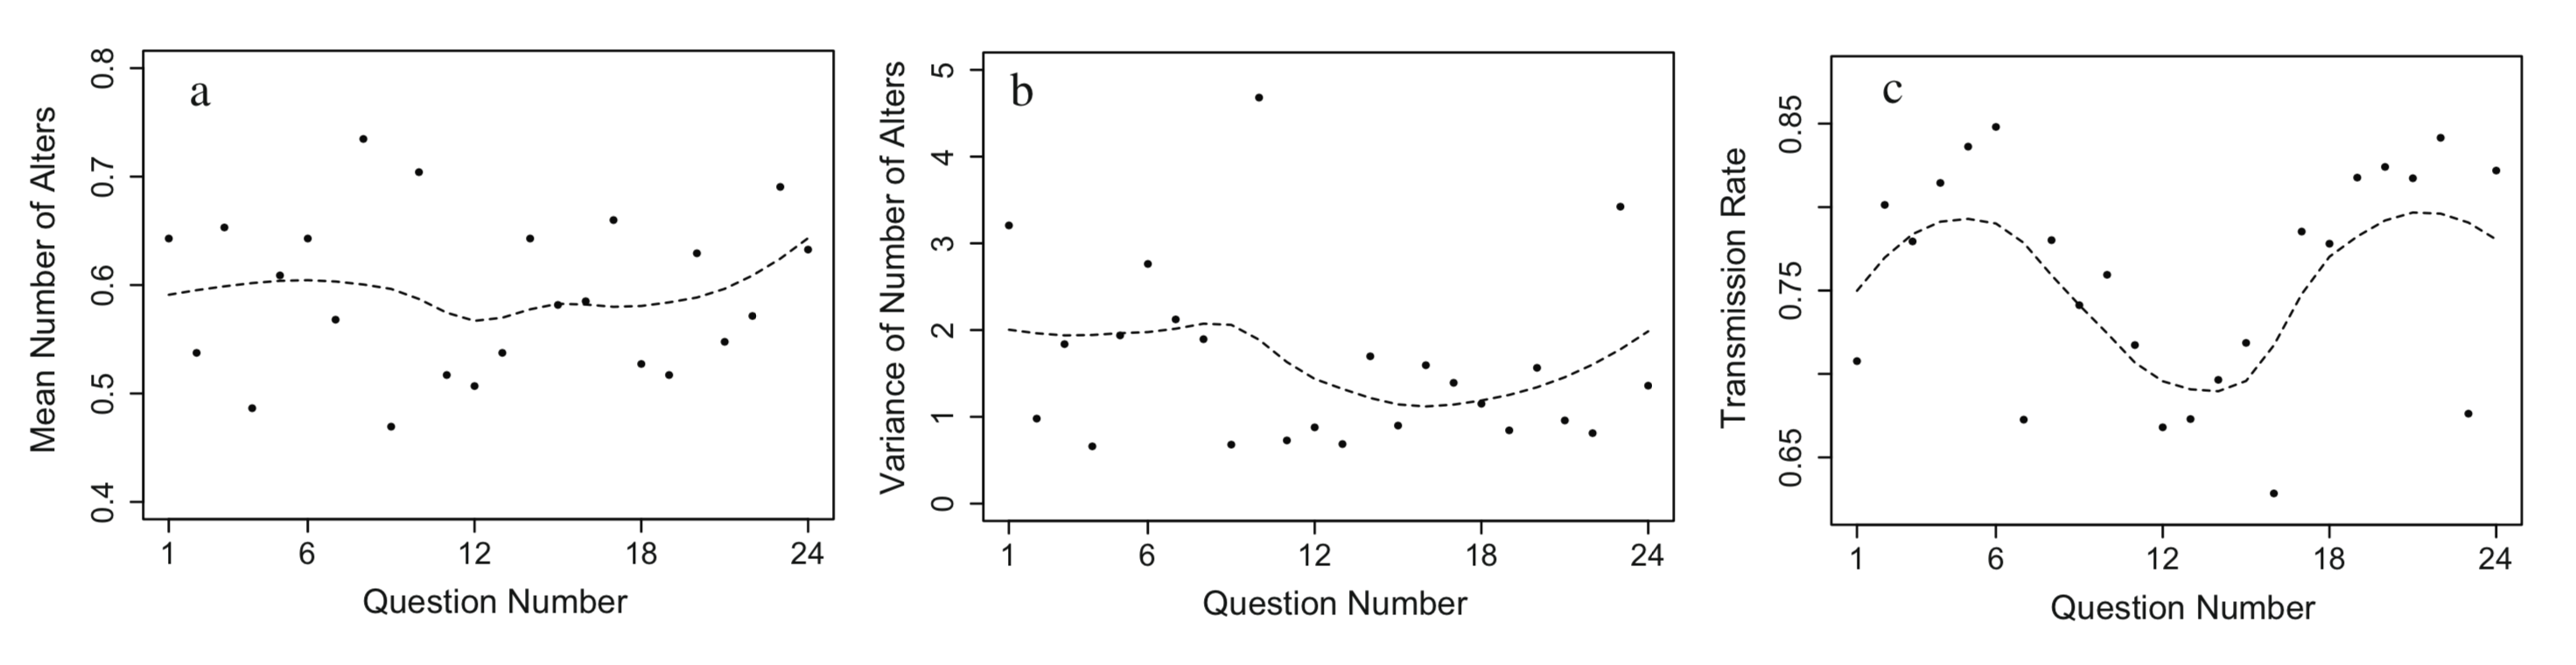
\includegraphics[width=\textwidth]{figures/salganik_game_2011_fig6}
\end{center}

\begin{itemize}
\item No strong evidence of question order effects
\end{itemize}

\end{frame}
%%%%%%%%%%%%%
\begin{frame}

\begin{center}	
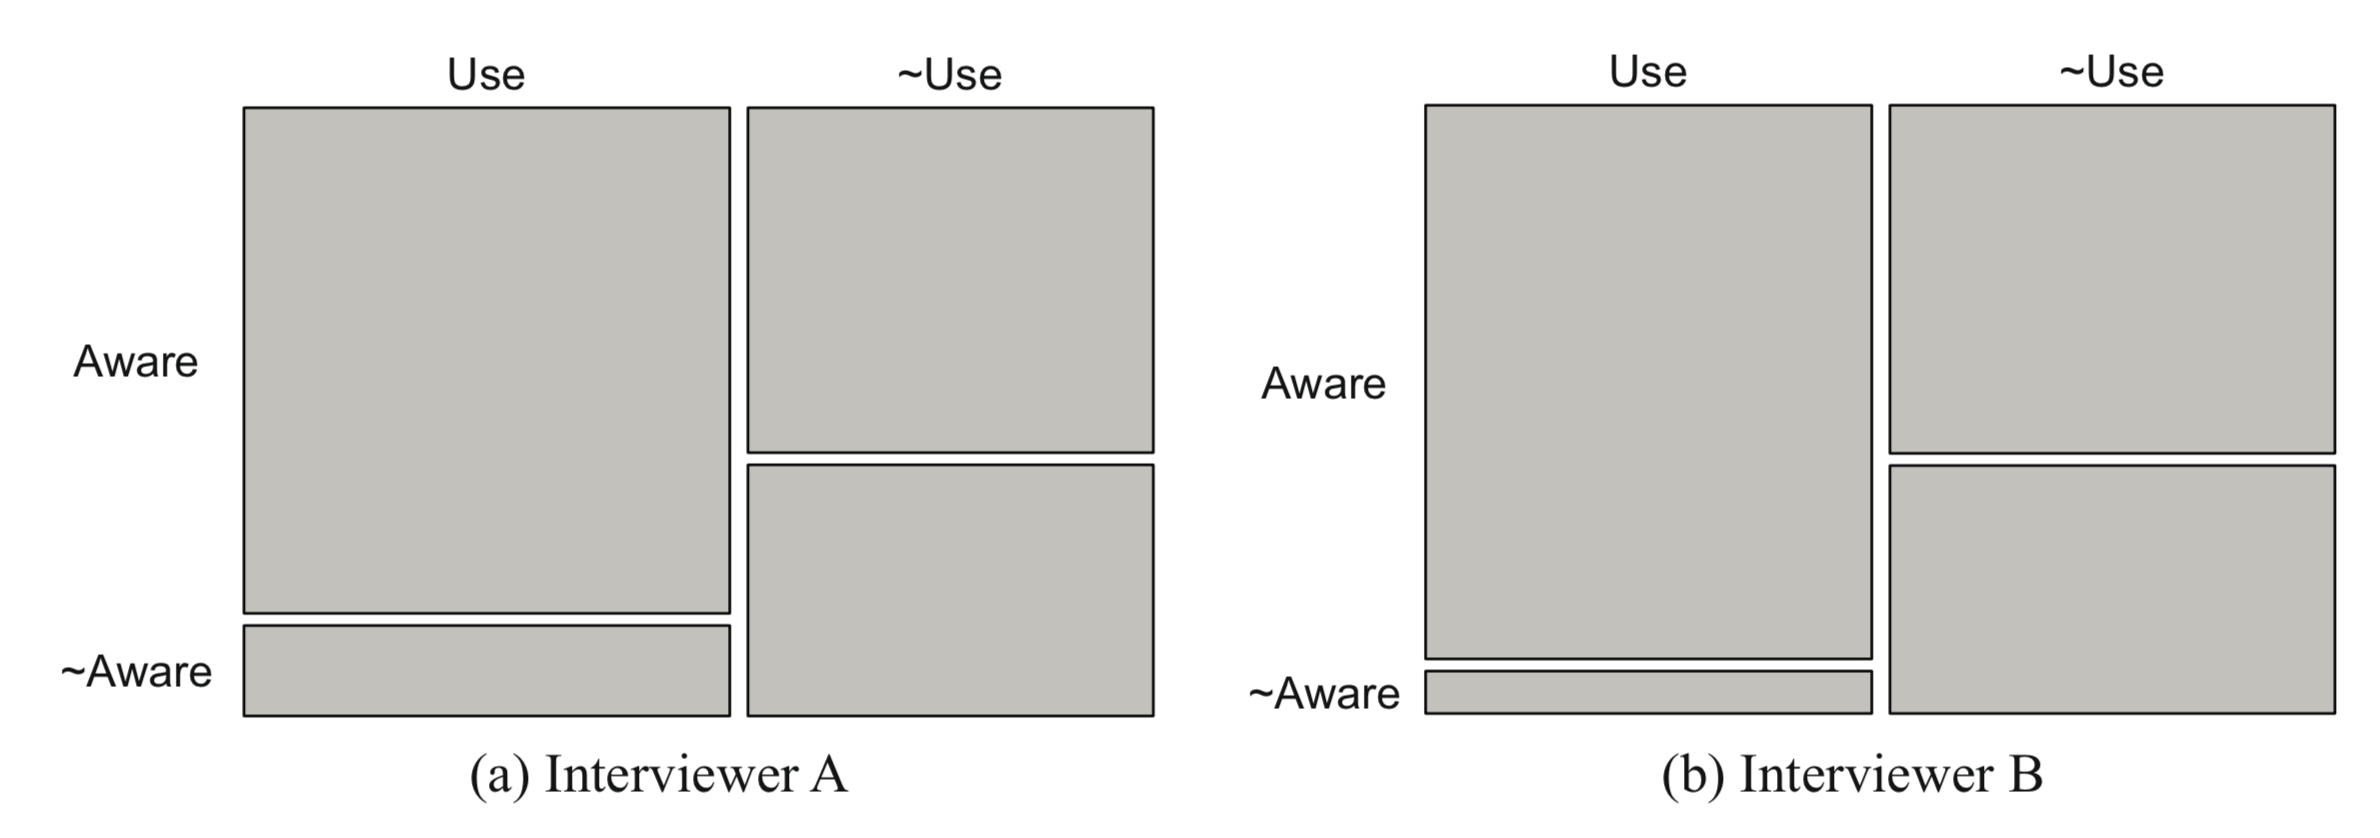
\includegraphics[width=\textwidth]{figures/salganik_game_2011_fig7}
\end{center}

\begin{itemize}
\item No strong interviewer effects
\end{itemize}

\end{frame}
%%%%%%%%%%%%%
\begin{frame}

We want to learn about:
\begin{itemize}
\item true positive rate (probability that a randomly chosen alter of a randomly chosen ego in the hidden population is aware that ego is in the hidden population) \pause
\end{itemize}

\vfill 
Bonus: we can combine this data with data from the general population to learn about the degree ratio (the difference in average network size between the hidden population and general population)

\end{frame}
%%%%%%%%%%%%%%
\begin{frame}

\begin{center}	
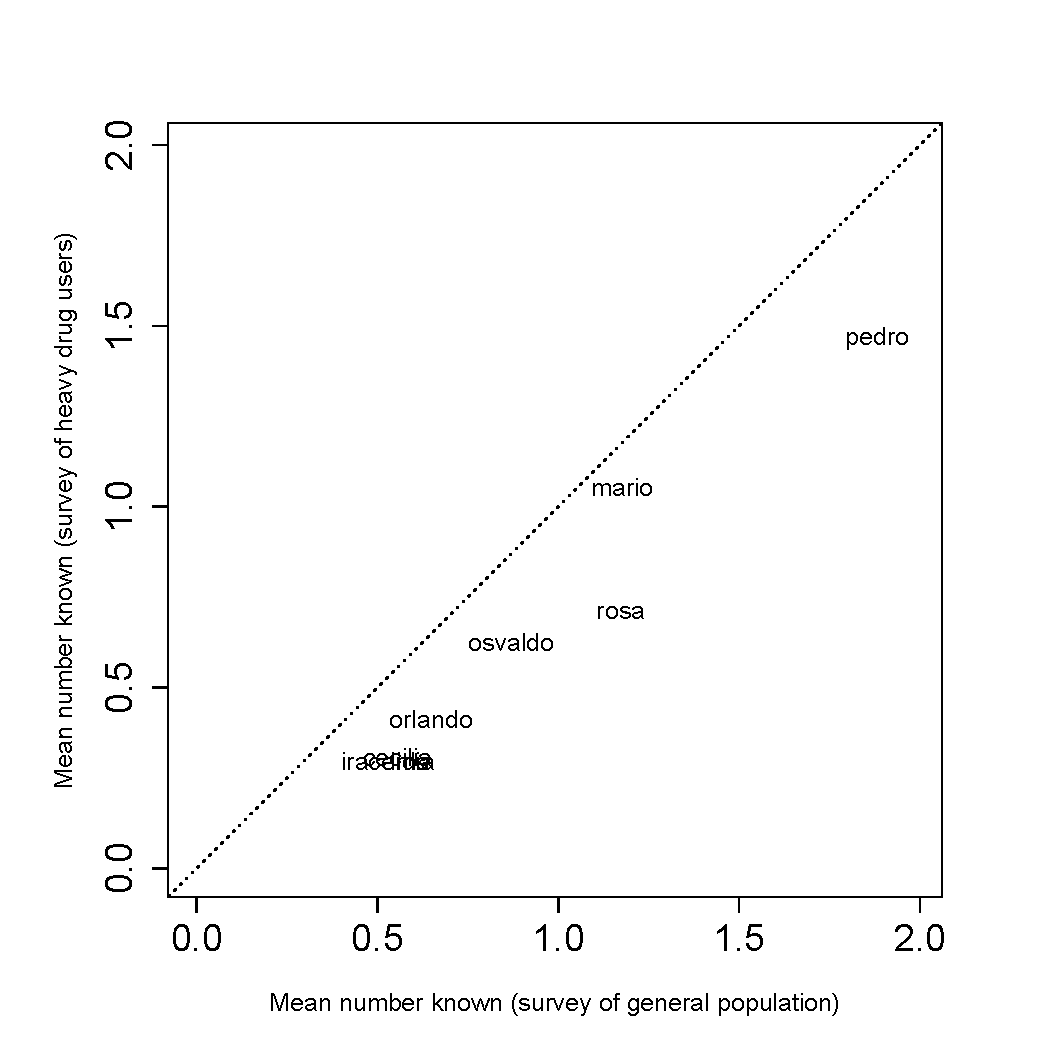
\includegraphics[width=0.4\textwidth]{figures/degreeratio_names}
\end{center}

Degree ratio is 0.69.  People in the hidden population have smaller personal networks that people in the general population

\end{frame}
%%%%%%%%%%%%%%%%%
\begin{frame}

\begin{align*}
\hat{\bar{v}}_{H,F} & = \hat{\bar{d}}_{F,F}  \times \underbrace{ \widehat{ \frac{ \bar{d}_{H,F} } { \bar{d}_{F,F} } } }_{\text{degree ratio ($\delta$)}} \times \underbrace{ \widehat{ \frac{ \bar{v}_{H,F} } { \bar{d}_{H,F} } } }_{\text{true positive rate ($\tau$)}} \\
\hat{\bar{v}}_{H,F} & = 184 \; \times \quad \; \; 0.69 \quad \; \; \times \quad \qquad 0.77 \quad \qquad \approx 100
\end{align*}

Average visible degree of the hidden population is very different from the average degree of the population

\end{frame}
%%%%%%%%%%%%%%%%%%%
\begin{frame}

How else can we study who knows what about who and what impacts that might have on individuals and groups?

\end{frame}


\end{document}
